\begin{frame}{Vegetationsstriber}

\small

\begin{columns}[T]

\begin{column}{0.58\textwidth}

\textbf{Regler ved vegetationsstriber:}

\begin{itemize}[]
\item Etableres langs søer, vandløb  og lign.
\item Uddyrket eller vildt- og bivenlig vegetation
\item Må ikke isås med kulturgræsser
\item Min. 3 m bred
\item Må ikke gødskes eller sprøjtes
\item Ved 3- og 5-årige biotopplaner: maks. 30\% af tiltaget omlægges årligt
\end{itemize}

\vspace{0.4em}

\textbf{Gavner arter:}

\footnotesize
Agerhøne, fasan, hare, rådyr, dådyr, sanglærke, vibe, gul vipstjert, 
rødrygget tornskade, gulspurv, vilde bier, humlebier, dagsommerfugle, 
rovbiller, græshopper, markmus, pindsvin, lækat, flagermus, musvåge, tårnfalk

\end{column}

\begin{column}{0.40\textwidth}
\centering
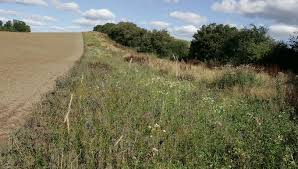
\includegraphics[width=\textwidth]{Billeder/Vildtforvaltning/biotopplantiltag/vegetationsstribe.jpeg}
\end{column}

\end{columns}

\end{frame}